% Bismillahi-r-Rahmani-r-Rahim
\documentclass{article}
\author{Daoud Clarke}
\date{\today}
\title{Investigations into New Lattice Orderings}

\usepackage{color}
\usepackage{graphicx}
\usepackage[round]{natbib}

\newtheorem{definition}{Definition}

\begin{document}

\maketitle

Context-theoretic semantics \citep{Clarke:07} defines a lattice
ordering on the vector space formed from contexts of words. The
lattice meet and join are defined by taking component-wise minimums
and maximums with respect to the basis defined by contexts: there is a
basis vector (dimension) for each context a word can occur in.

However, this ordering is only one that is possible on the vector
space. Here we consider two others and evaluate their plausibility for
defining entailment between vector representations of meaning.

\section{Motivation}

In \citep{Clarke:12}, a context theory is defined as follows:
\begin{definition}[Context Theory]
A context theory is a tuple $\langle A, \mathcal{A}, \xi, V, \psi
\rangle$, where $A$ is a set (the alphabet), $\mathcal{A}$ is a unital
algebra over the real numbers, $\xi$ is a function from $A$ to
$\mathcal{A}$, $V$ is an abstract Lebesgue space and $\psi$ is an
injective linear map from $\mathcal{A}$ to $V$.
\end{definition}

The definition is quite complex because the space $V$ in which the
ordering is defined is a bigger space than the space $\mathcal{A}$
used to define composition. If we were able to define an ordering on
$\mathcal{A}$ instead, then this would significantly simplify the
definition, to $\langle A, \mathcal{A}, \xi\rangle$.

\section{Background}

A \textbf{partially ordered vector space} is a vector space $V$
together with a partial ordering $\le$ that satisfies:
\begin{itemize}
\item If $u \le v$ then $u + w \le v + w$
\item If $u \le v$ then $\alpha u \le \alpha v$
\end{itemize}
for all $u,v,w \in V$ and $\alpha \ge 0$. If the partial ordering is a
lattice, then the vector space is called a vector lattice or
\textbf{Riesz space}.

\begin{center}
%% Creator: Inkscape inkscape 0.48.0, www.inkscape.org
%% PDF/EPS/PS + LaTeX output extension by Johan Engelen, 2010
%% Accompanies image file 'cones.pdf' (pdf, eps, ps)
%%
%% To include the image in your LaTeX document, write
%%   \input{<filename>.pdf_tex}
%%  instead of
%%   \includegraphics{<filename>.pdf}
%% To scale the image, write
%%   \def\svgwidth{<desired width>}
%%   \input{<filename>.pdf_tex}
%%  instead of
%%   \includegraphics[width=<desired width>]{<filename>.pdf}
%%
%% Images with a different path to the parent latex file can
%% be accessed with the `import' package (which may need to be
%% installed) using
%%   \usepackage{import}
%% in the preamble, and then including the image with
%%   \import{<path to file>}{<filename>.pdf_tex}
%% Alternatively, one can specify
%%   \graphicspath{{<path to file>/}}
%% 
%% For more information, please see info/svg-inkscape on CTAN:
%%   http://tug.ctan.org/tex-archive/info/svg-inkscape

\begingroup
  \makeatletter
  \providecommand\color[2][]{%
    \errmessage{(Inkscape) Color is used for the text in Inkscape, but the package 'color.sty' is not loaded}
    \renewcommand\color[2][]{}%
  }
  \providecommand\transparent[1]{%
    \errmessage{(Inkscape) Transparency is used (non-zero) for the text in Inkscape, but the package 'transparent.sty' is not loaded}
    \renewcommand\transparent[1]{}%
  }
  \providecommand\rotatebox[2]{#2}
  \ifx\svgwidth\undefined
    \setlength{\unitlength}{259pt}
  \else
    \setlength{\unitlength}{\svgwidth}
  \fi
  \global\let\svgwidth\undefined
  \makeatother
  \begin{picture}(1,0.71832129)%
    \put(0,0){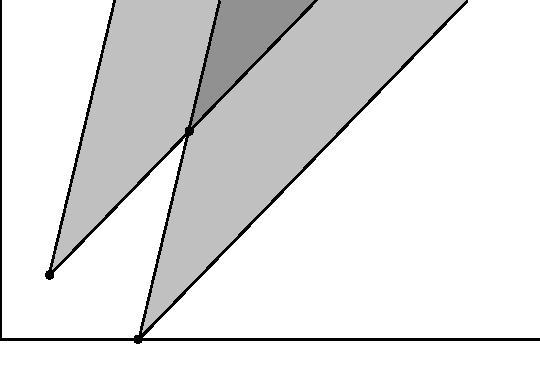
\includegraphics[width=\unitlength]{cones.pdf}}%
    \put(0.0289539,0.14386651){\color[rgb]{0,0,0}\makebox(0,0)[lb]{\smash{$u$}}}%
    \put(0.20731187,0.01815878){\color[rgb]{0,0,0}\makebox(0,0)[lb]{\smash{$v$}}}%
    \put(0.32271158,0.41831799){\color[rgb]{0,0,0}\makebox(0,0)[lb]{\smash{$u\lor v$}}}%
  \end{picture}%
\endgroup

\end{center}

A \textbf{cone} is a subset $C$ of a vector space satisfying
\begin{itemize}
\item $C + C \subseteq C$
\item $\alpha C \subseteq C$ for all $\alpha \ge 0$
\item $C \cap (-C) = \{0\}$
\end{itemize}
If $V$ is a partially ordered vector space, then the set $V^+ = \{v
\in V : v \ge 0\}$ is a cone, called the \textbf{positive
  cone}. Conversely, given any cone $C$ for a vector space $V$, we can
define a partial ordering on $V$ by $u \le v$ iff $v - u \in C$.

Given a countable set $U = \{u_1, u_2, \ldots\}$ of vectors, the cone
generated by $U$ is the set $C_U = \{v : v = \sum_i \alpha_i u_i\}$ for
some $\alpha_i \ge 0$.

\section{Context Vector Cones}

We can define a positive cone on $\mathcal{A}$ to be the cone
generated by all context vectors, $\hat{A} = \{\hat{x} : x \in A^*\}$. There are
two questions we can ask:
\begin{itemize}
\item Is the ordering interesting, or is likely to turn out to be
  trivial (for example, all strings have meet $0$)?
\item Does the ordering define a lattice? We need the meet operation
in order to define a degree of entailment between strings.
\end{itemize}

In fact it seems that we can't have our cake and eat it, as if the
first question is true, it seems likely the second is false, and vice
versa. If the set $\hat{A}$ is linearly independent, then it seems
that the first is true, and the second false, while the converse holds
in general otherwise. (At the moment, I only have an intuition for
this --- I've yet to prove it).


\section{Plane Orderings}

\bibliographystyle{plainnat}

\bibliography{contexts}

\end{document}
